\section{Performance comparison}
\label{sec:performance_comparison}

In this section we present some results obtained using the described robust planning frameworks. All planned trajectories refer to the sector of the Catalunya circuit shown in Fig.~\ref{fig:track}.
The entire circuit is parameterized by the curvilinear parameter $\alpha \in [0,1]$, and the selected sector corresponds to the interval $\left[0.70, 0.77\right]$. Checkpoints are indicated by labels and are uniformly spaced by $\De\al=0.01$. This sector includes two distinct corners: a low-speed turn from $\al = 0.72$ to $\al = 0.73$, and a high-speed turn from $\al = 0.75$ to $\al = 0.76$, allowing for the evaluation of vehicle behavior across different dynamic scenarios.

First we present selected results from the open-loop planning, which helps illustrate the method and its underlying mechanism. 
%We begin by presenting a selection of results obtained with the open-loop planning approach, which allows for a clearer illustration of the method and its underlying mechanisms. 
This serves as a reference to assess the impact of key design parameters and constraint types on planned trajectories.
We then compare open- and closed-loop strategies, and finally validate the framework by comparing planned trajectories and simulations with noise realization.
%A comparison is then carried out between the open-loop and closed-loop strategies. Finally, the planned trajectories are compared against those followed in simulations with noise realizations, providing empirical validation of the proposed framework.

The chosen sector was discretized into 140 spatial intervals ($\De s$ = 0.43 m). Both the open- and closed-loop disturbance-aware planning problems were transcribed on this grid in the CasADi-MATLAB environment~\cite{Andersson:MPC:2019}, and the resulting nonlinear programs were solved with IPOPT's interior-point algorithm~\cite{Wachter:MP:2006}.
  

% Contour plot dei LAP time in funzione dei due gamma, lo mettiamo o no? Eventialmente nel comparison open/closed

\begin{figure}
	\centering
	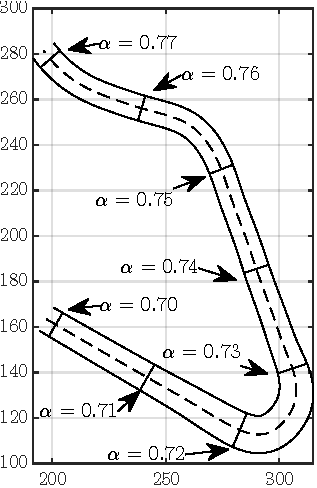
\includegraphics{Fig/track.pdf}
	\caption{The analyzed Catalunya circuit sector spans $\alpha \in [0.70, 0.77]$, with labeled checkpoints every $\Delta\alpha = 0.01$. It contains two corners -- a low-speed turn ($\alpha = 0.72-0.73$) and a high-speed turn ($\alpha = 0.75-0.76$) -- providing contrasting dynamic conditions for vehicle behavior evaluation.}
	\label{fig:track}
\end{figure}

\subsection{Open-loop parameter sensitivity}
\label{sec:ol_param_sensitivity}
To better understand the effect of key parameters, we focus on the open-loop formulation with robustified track limit constraint. This choice favors clearer visual interpretation.
%To gain deeper insight into how key parameters affect the planning outcome, we focus here on the open-loop formulation. At this stage, only the track limit constraint is robustified. This choice is motivated by the fact that its effects are more visually evident than those of the friction limit constraint, thereby facilitating a more immediate understanding of their impact.
The first parameter considered is the confidence level of constraint satisfaction.
We recall that the factor $\ga^\textrm{TLC}$ acts as a tuning knob, multiplying the standard deviation of the constraint, $\sigma^\textrm{TLC}$, to determine the total back-off term $\be^\textrm{TLC}$.
This parameter directly influences the probability of satisfying the track limit constraint: higher values of $\ga^\textrm{TLC}$ correspond to more conservative (i.e., robust) behavior.
Specifically, $\ga^\textrm{TLC} = 0$ yields a satisfaction probability of 50\% and leads to the nominal solution with no back-off, while $\ga^\textrm{TLC} = 3$ corresponds to a confidence level of 99\%.
%For the purposes of this analysis, we examine the effect of varying $\ga^\textrm{TLC}$ in this range.

%Setting $\ga^\textrm{TLC} = 0$ leads to the nominal solution. In this case, the back-off term $\be^\textrm{TLC}$ becomes zero, meaning that the constraint is not robustified and thus coincides with the original, non-robust formulation.

As shown in the left panel of Fig.~\ref{fig:ol_sensitivities}, trajectories with lower values of $\ga^\textrm{TLC}$ (darker blue) yield smaller lateral margins with respect to the track boundaries. In contrast, the trajectory with $\ga^\textrm{TLC} = 3$ (light green) remains noticeably farther from the edges.
This behavior is consistent with the increased conservativeness introduced by higher values of $\ga^\textrm{TLC}$, which amplify the back-off term $\be^\textrm{TLC}$ and thereby enforce a larger safety margin from the track limits.
Larger safety margins lead to higher sector times; spanning $\ga^\textrm{TLC}$ in the range $\left[0,3\right]$ results in sector times that vary from 12.135\,s to 13.162\,s.

\begin{figure}
	\centering
	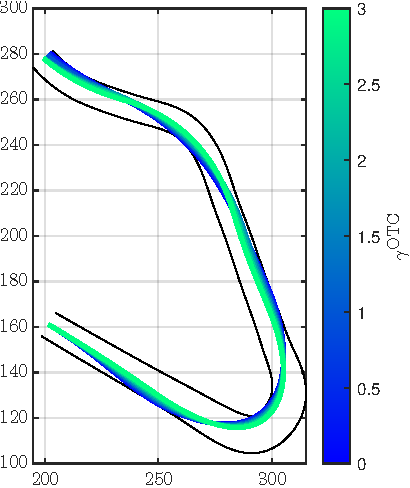
\includegraphics{Fig/gamma_sensitivity.pdf}
	\hfill
	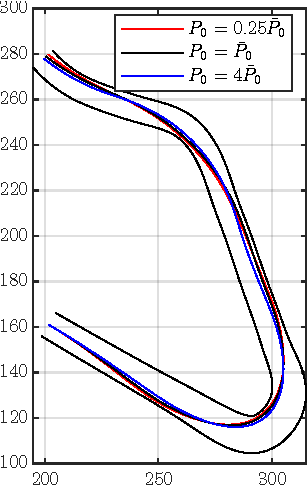
\includegraphics{Fig/Pzero_sensitivity.pdf}
\caption{Effect of the TLC penalty coefficient $\gamma^{\mathrm{TLC}}$ (left panel) and the initial covariance $\mathbf P_{0}$ (right panel) on the optimal trajectory.
Raising $\gamma^{\mathrm{TLC}}$ from 0 to 3 increases the probability of satisfying the track-limit constraints from 50 \% to 99 \%.
The right panel compares the nominal covariance $\bar{\mathbf P}_{0}$ (black) with $4\bar{\mathbf P}_{0}$ (blue line) and $\tfrac14\,\bar{\mathbf P}_{0}$ (red line), i.e., twice and half the nominal state uncertainty.
}
%\caption{Effect of $\ga^\textrm{TLC}$ (left panel) and $\bP_0$ (right panel) on optimal trajectory. The parameter $\ga^\textrm{TLC}$ spans in the range $\left[0,3\right]$ corresponding to a probability to meet the track limit constraint ranging from 50\% to 99\%. In the right panel, in addition to the baseline value $\bar{\bP}_0$ (black line), two alternative values are considered: $\bP_0 = 4\bar{\bP}_0$ (blue line) and $\bP_0 = \frac{1}{4}\bar{\bP}_0$ (red line). These correspond, respectively, to doubling and halving the initial uncertainty associated with the state vector.}
	\label{fig:ol_sensitivities}
\end{figure}

The second parameter examined is the initial value of the covariance matrix $\bP_0$.
We recall that at each grid point a new prediction horizon is initialized, and the corresponding matrix $\bP$ at its starting point, i.e., $\bP^0_k$, is set to $\bP_0$.
The diagonal elements of $\bP$ are the variances $\Var{x_i}$  of each state variable, while the off-diagonal elements encode their covariances $\Cov{x_i}{x_j}$. Larger diagonal values indicate higher uncertainty in the corresponding states, and nonzero off-diagonal terms imply mutual dependence between them. For simplicity, a diagonal $\bP_0$ is used in this study, that is, for each prediction horizon we assign an initial standard deviation $\sig_{x_i}$ to each state and assume all initial covariances $\Cov{x_i}{x_j}$  to be zero.

 Assuming the state vector is ordered as described in Section~\ref{sec:vehicle_model}, the baseline initial covariance matrix is set to $\bP_0=\diag(\bbsig^2)$, with
\begin{align}
\bar{\boldsymbol{\sigma}}~=~\left[0.1\,\textrm{m/s}, 0.01\,\textrm{m/s}, 0.01\,\textrm{rad/s}, 1\,\textrm{m}, 1\,\textrm{m}, 0.0175\,\textrm{rad}\right]^T.
\end{align}
These standard deviations have been chosen based on the typical range of variation of each state. To provide a concrete interpretation at the starting condition, the assumption on first state $u \sim \calN(\mu_u,\sig_u^2)$, with $\sig_u=0.1$ m/s, implies that
$\Pr\{\mu_u-\sig_u \leq u \leq \mu_u+\sig_u\}\approx 68\%$ and $\Pr\{\mu_u-3\sig_u \leq u \leq \mu_u+3\sig_u\}\approx 99\%$.

In addition to the baseline value $\bar{\bP}_0$, two alternative values are considered: $\bP_0 = 4\bar{\bP}_0$ and $\bP_0 = \frac{1}{4}\bar{\bP}_0$. These correspond, respectively, to doubling and halving the initial standard deviations $\sig_{x_i}$ associated with each state vector.

A comparison between the trajectories obtained using different values of $\bP_0$ is shown in the right panel of Fig.~\ref{fig:ol_sensitivities}.
The black line corresponds to the baseline case with $\bP_0 = \bar{\bP}_0$, while the red and the blue lines represent the cases with $\bP_0 = \frac{1}{4}\bar{\bP}_0$ and $\bP_0 = 4\bar{\bP}_0$, respectively. As reasonably expected, using a larger initial covariance matrix results in an inflated covariance matrix that reflects increased uncertainty after $H$ steps, which in turn leads to a higher back-off term. This is associated to the blue line, which travels closer to the centerline with respect to the other two lines.

\subsection{Open-Loop vs. Closed-Loop comparison}

\begin{figure}[t]
	\centering
	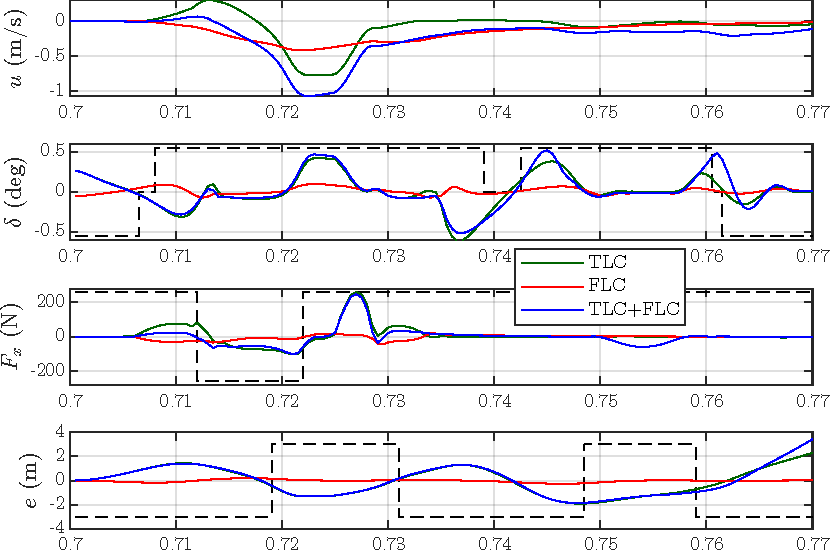
\includegraphics{Fig/ol_telemetries.pdf}
	\caption{Open-Loop method. Variations of longitudinal speed $\Delta u$, steering angle $\Delta\delta$, longitudinal force $\Delta F_x$, and lateral deviation $\Delta e$ relative to the nominal trajectory for three schemes --- TLC (track-limit), FLC (friction-limit), and TLC+FLC (both).
	Dashed lines mark the sign of the reference signal (positive, near-zero and negative).}
	
	%\caption{Evolution of the longitudinal speed $\De u$, wheel steering angle $\De \de$, longitudinal force $\De F_x$, and lateral deviation $\De e$ are reported for three robustification scenarios: TLC (Track Limit Constraints), FLC (Friction Limit Constraint), and TLC+FLC (both constraints enforced concurrently). Each profile is shown relative to the baseline (nominal) trajectory to highlight the effect of each constraint-handling strategy. The dashed lines in the last three panels indicate the sign of the reference signal, allowing one to determine whether a positive variation with respect to the baseline corresponds to an increase or a decrease in the absolute value. This distinction is particularly important for quantities that depend on the direction of the turn, such as the wheel steering angle $\de$ and the lateral deviation $e$, while in the case of $F_x$, it indicates whether the vehicle is accelerating or braking.}
	\label{fig:ol_telemetries}
\end{figure}

\begin{figure}[t]
	\centering
	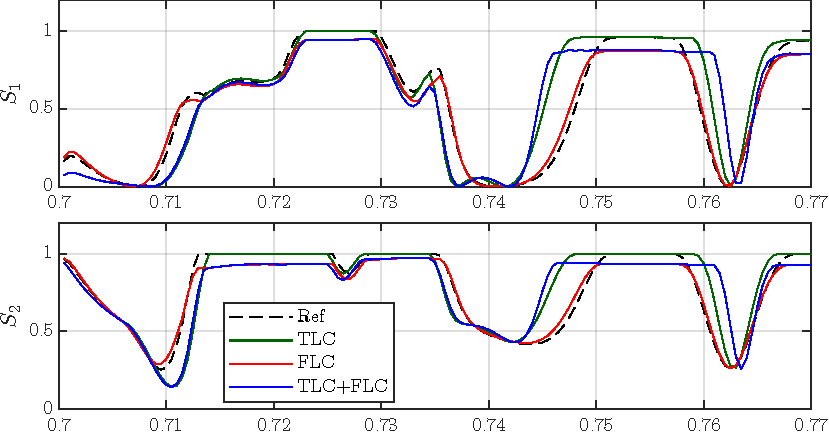
\includegraphics[scale = 1]{Fig/ol_saturation.pdf}
	\caption{Open-Loop. Axle saturation $S_j(\bx,\bu)$ for front axle (j=1, first panel) and rear axle (j=2, second panel) with respect to the curvilinear parameter $\al$. Nominal configuration in dashed black, TLC in green, FLC in red, TLC+FLC in blue.
	%The dashed black line corresponds to the reference (nominal) configuration, while the green, red, and blue lines represent the robustified configurations TLC, FLC, and TLC+FLC, respectively.
	}
	\label{fig:ol_saturation}
\end{figure}

%It is of interest to analyze how a robustified constraint---or a combination of the two described in Sections~\ref{sec:FLC} and~\ref{sec:TLC}---influences the driving style.
We now investigate how the inclusion of different kinds of robustified constraints --- individually or in combination, as described in Sections~\ref{sec:FLC} and~\ref{sec:TLC} --- influences the driving style.
We compare the nominal feed-forward optimal trajectory, obtained without robustified constraints, with those resulting from a robustified track limit constraint (denoted as TLC), a robustified friction limit constraint (denoted as FLC), and a scenario where both constraints are robustified (denoted as TLC+FLC).

First we show results obtained with the open-loop method described in Section~\ref{sec:open_loop_planning}, setting $H=4$, and $\ga^\textrm{TLC}=\ga^\textrm{FLC}=1.28$, corresponding to a 90\% probability of satisfying both constraints.
%All the optimization are obtained with the open-loop method described in Section~\ref{sec:open_loop_planning}, setting $H=4$, and $\ga^\textrm{TLC}=\ga^\textrm{FLC}=1.28$, corresponding to a 90\% probability of satisfying both constraints.
%---Delta key signals
The comparison between the nominal case and the three robustified cases is illustrated in Fig.~\ref{fig:ol_telemetries}, in terms of the deviation of selected signals from to their nominal counterparts.
The panels display variations on the longitudinal speed $\De u$ (first panel), wheel steering angle $\De \de$ (second panel), total longitudinal force $\De F_x$ (third panel), and lateral deviation of the center of mass (CoM) from the track centerline $\De e$ (fourth panel).
Except for the $\De u$ panel, each plot includes dashed black lines that indicate the sign of the nominal signal.
These indicators are shown at three distinct vertical levels --- high, medium, and low --- corresponding respectively to positive, near-zero, and negative values of the nominal signal.

%--------1 Considerazioni generali sul settore

From the first panel, it can be observed that all robustified configurations, on average, show a lower longitudinal speed compared to the nominal trajectory, resulting in an increased sector time. Specifically, the configuration with the robustified TLC increases the sector time by 1.66\%, while that with the robustified FLC leads to a 0.79\% increase. When both TLC and FLC are robustified, the sector time increases by 2.57\%.
The two configurations incorporating the robustified TLC (blue and green lines) exhibit, as expected, a significantly altered CoM trajectory.
Indeed, the second and fourth panels clearly show that the TLC and TLC+FLC configurations tend to follow a path closer to the centerline. In particular, for most of the sector, the variation in lateral displacement $\De e$ and the lateral displacement $e$ itself exhibit opposite signs, indicating a corrective behavior of the steering angle $\de$ that pulls the vehicle toward the centerline.

%--------2 Sharp turn

This shift in trajectory and longitudinal speed becomes especially evident when approaching the sharp turn for $\al \in [0.707, 0.712]$. A noticeable increase in longitudinal speed is observed around $\alpha = 0.71$ for the TLC configuration  in the $\De u$ panel. This peak is followed by a sharp drop in speed, indicating intense braking.
The TLC+FLC configuration demonstrates a qualitatively similar trend in $\Delta u$, although the peak is significantly lower and the subsequent speed reduction is clearly stronger. This behavior is consistent with the variation of the total longitudinal force $\Delta F_x$ shown in the third panel.
%\textcolor{red}{In particular, the TLC and TLC+FLC configurations exhibit a higher longitudinal force while approaching the sharp turn, in the curvilinear abscissa interval $\al\in\left[0.707, 0.712\right]$, resulting in a higher longitudinal speed.
%Subsequently, these two configurations apply a lower longitudinal force during braking compared to the nominal case, indicating more intense braking. This behavior explains the sharp reduction in longitudinal speed observed thereafter.}

%--------3 High speed turn

Later in the sector, a further deviation in driving style appears during the high-speed turn, specifically around $\alpha \in [0.75, 0.76]$.
As shown in the third panel ($\Delta F_x$), in the combined configuration TLC+FLC a reduction in the longitudinal force within this sector is needed to meet both constraints.
This adaptation is necessary because the TLC forces the vehicle to follow a wider trajectory, which entails greater lateral acceleration and, consequently, higher lateral force demand. To satisfy the FLC under the resulting increase in tire utilization, the available accelerating force must be reduced.
Based on the nominal force sign indicator, this reduction is achieved by partially lifting the throttle.

%---Axle saturation
After analyzing the variations of these four key signals with respect to the nominal solution, we now turn our attention to the evaluation of axle saturation $S_j(\bx,\bu)$ defined in Eq.~\eqref{eq:axle_saturation}, which provides insight into how close each configuration operates to the tire grip limits.

Figure~\ref{fig:ol_saturation} shows the values of $S_j(\bx,\bu)$ for the front axle ($j=1$, first panel) and the rear axle ($j=2$, second panel) for the previously introduced configurations: the nominal case (black dashed line) and the three robustified cases TLC, FLC and TLC+FLC (color-coded as before).

Firstly, we observe that the FLC and TLC+FLC configurations (red and blue lines) never reach full saturation ($S_j=1)$ due to the presence of the back-off term, which enforces a safety margin from the friction limit.
Secondly, we point out how the different trajectories followed by the TLC and TLC+FLC configurations (green and blue lines), compared to the nominal (black) and FLC case (red), entail distinct ground force demands, which are clearly visible here in terms of the $S_j$ ratio.
This behavior emerges around the sharp turn and becomes even more evident in the high-speed turn.
Specifically, in the interval $\al \in [0.745, 0.762]$, the TLC and TLC+FLC configurations begin to experience high axle loads approximately 12\,m before the nominal trajectory and sustain them for an additional 4.6\,m (TLC, green line) and 9.2\,m (TLC+FLC, blue line) beyond the nominal reference.

%As already observed, the configurations with the robustified track limit constraint (green and blue lines) follow significantly different paths compared to the nominal solution. This deviation results in distinct ground force demands, clearly visible in the saturation index.
%From this plot, it can be observed that the configurations with the robustified track limit constraint (green and blue lines) follow significantly different trajectories compared to the nominal solution, resulting in distinct ground force demands. This behavior is noticeable in turn 1 and even more clearly in turn 2. Specifically, these two configurations begin to experience high axle loads approximately 12\,m before the nominal trajectory and sustain them for an additional 4.6\,m (TLC, green line) and 9.2\,m (TLC+FLC, blue line) beyond the nominal reference.

\begin{figure}[t]
	\centering
	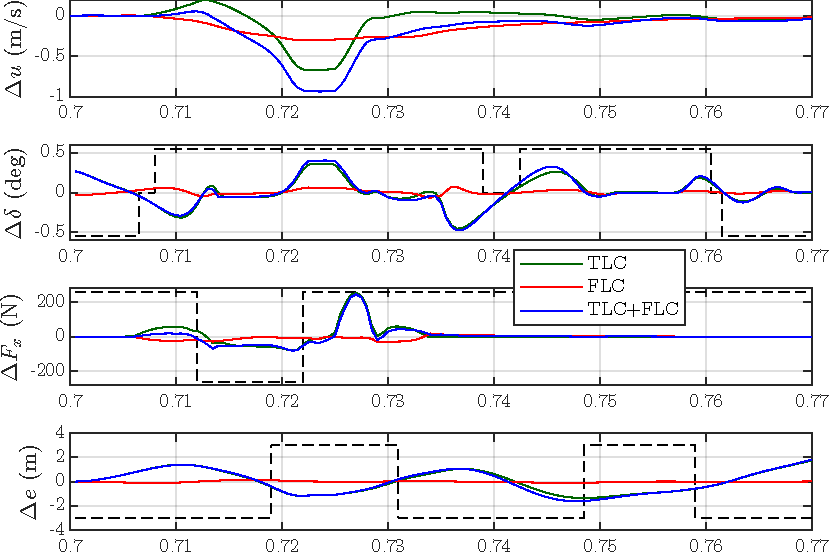
\includegraphics{Fig/cl_telemetries.pdf}
	\caption{Closed-Loop method. Variations of longitudinal speed $\De u$, steering angle $\De\de$, longitudinal force $\De F_x$, and lateral deviation $\De e$ relative to the nominal trajectory for three schemes --- TLC (track-limit), FLC (friction-limit), and TLC+FLC (both).
		Dashed lines mark the sign of the reference signal (positive, near-zero and negative).}
	
	%\caption{Evolution of the longitudinal speed $\De u$, wheel steering angle $\De \de$, longitudinal force $\De F_x$, and lateral deviation $\De e$ are reported for three robustification scenarios: TLC (Track Limit Constraints), FLC (Friction Limit Constraint), and TLC+FLC (both constraints enforced concurrently). Each profile is shown relative to the baseline (nominal) trajectory to highlight the effect of each constraint-handling strategy. The dashed lines in the last three panels indicate the sign of the reference signal, allowing one to determine whether a positive variation with respect to the baseline corresponds to an increase or a decrease in the absolute value. This distinction is particularly important for quantities that depend on the direction of the turn, such as the wheel steering angle $\de$ and the lateral deviation $e$, while in the case of $F_x$, it indicates whether the vehicle is accelerating or braking.}
	\label{fig:cl_telemetries}
\end{figure}
\begin{figure}[b!]
	\centering
	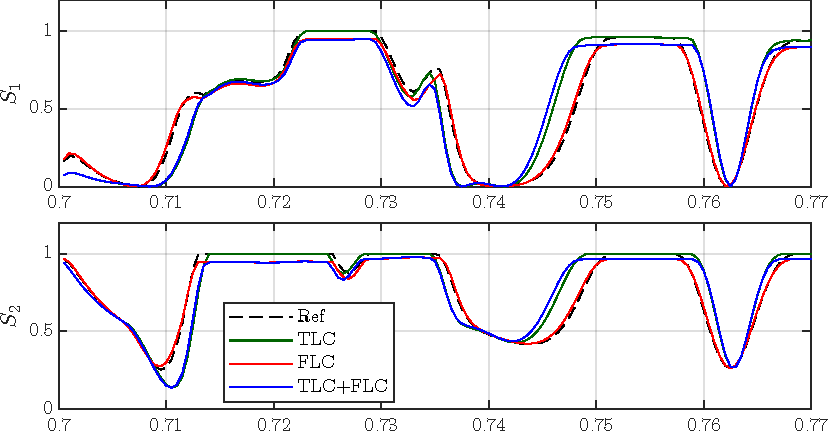
\includegraphics[scale = 1.005]{Fig/cl_saturation.pdf}
	\caption{Closed-Loop. Axle saturation $S_j(\bx,\bu)$ for front axle (j=1, first panel) and rear axle (j=2, second panel) with respect to the curvilinear parameter $\al$. Nominal configuration in dashed black, TLC in green, FLC in red, TLC+FLC in blue.
		%The dashed black line corresponds to the reference (nominal) configuration, while the green, red, and blue lines represent the robustified configurations TLC, FLC, and TLC+FLC, respectively.
	}
	\label{fig:cl_saturation}
\end{figure}

An analogous analysis has been conducted using the closed-loop approach described in Section~\ref{sec:closed_loop_planning}, setting $\ga^\textrm{TLC}=\ga^\textrm{FLC}=1.28$.
The same key signals displayed for the previous case are shown in Fig.~\ref{fig:cl_telemetries}, while the axle saturation ratios $S_j$ are illustrated in Fig.~\ref{fig:cl_saturation}.
From one side, the results appear very similar to those obtained with the open-loop method. While the closed-loop method offers a more rigorous framework by enabling seamless covariance propagation over the entire lap, the observed agreement indicates that open-loop planning remains a valid and effective strategy, as long as the prediction horizon is appropriately selected.

On the other hand, the trajectories are also sufficiently different to appreciate some subtle but relevant distinctions. For instance, sector time increments w.r.t. the nominal case of corresponding configurations are lower than the ones arising from the open-loop method: 1.39\% for the TLC, 0.66\% for the FLC, and 2.07\% for the TLC+FLC.
Moreover, in both TLC and TLC+FLC configurations, the magnitude of $\De\de$ is appreciably smaller in the closed-loop case compared to the open-loop one, especially during the high-speed turn.
Additionally, the TLC+FLC configuration no longer exhibits the throttle release in $\De F_x$ observed in the open-loop case.

As for the axle saturation, both methods lead to qualitatively similar evolutions, but slight differences can be observed within the high-speed turn interval $\al \in [0.745, 0.762]$. In this case, the TLC and TLC+FLC configurations begin to experience high axle loads approximately 10\,m before the nominal trajectory and sustain them for an additional 4.5\,m beyond the nominal reference. This is achieved through the closed-loop method's capability to \emph{steer} and \emph{tame} the covariance matrix propagation via the dynamic action of the controller.

%\subsection{Open-loop vs closed-loop robust planning}
\begin{figure}[b!]
	\centering
	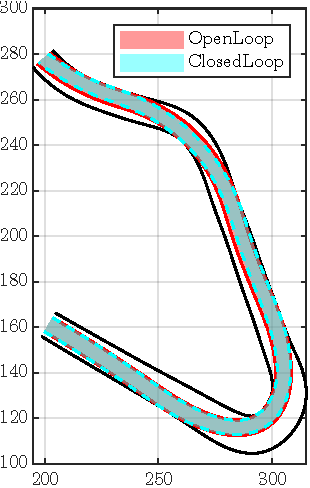
\includegraphics{Fig/olcl_traj_bands.pdf}
	\caption{Back-off envelopes for the open-loop (red) and closed-loop (cyan) robust planners. Each shaded band represents the area swept by the back-off-extended vehicle and must lie entirely within the actual track boundaries.
		The open-loop approach yields a wider envelope due to worst-case growth assumptions, whereas the closed-loop design, aided by time-varying LQR controller, maintains a narrower margin.}
	\label{fig:olcl_traj_bands}
\end{figure}

Finally, we compare the influence of the back-off terms on the open-loop and closed-loop trajectories, in the robustified TLC scenario with the high $\ga^\textrm{TLC}=3.0$ value for better visualization. As before, the open-loop planning is carried out with a prediction horizon of $H=4$ steps.
The back-off term $\be^{TLC}$ in Eq.~\eqref{eq:TLC} admits an interesting geometrical interpretation: it corresponds to the amount by which the track boundaries are (not uniformly) tightened to meet the probabilistic constraint, or, equivalently, to a virtual extension of the vehicle's width.

According to the latter interpretation, Fig.~\ref{fig:olcl_traj_bands} shows two highlighted bands---red for the open-loop case and cyan for the closed-loop case---corresponding to the area swept by the back-off-extended-vehicle. Ultimately, the TLC enforces precisely that these bands remain entirely within the actual track limits. The comparison between the two regions illustrates how the additional conservativeness of the open-loop approach stems from larger back-off terms, i.e., a wider band that must stay within the track boundaries. The closed-loop method, on the other hand, benefits from the LQR-based feedback, which allows it to maintain smaller back-off terms and thus a narrower band, requiring a reduced safety margin from the track limits.

% Solver times
Solver times (build time is negligible) were measured on a laptop equipped with an Intel Core i9-13980HX with 32 GB RAM.
The reference (nominal) plan, described in Sec.~\ref{sec:nominalFF}, contains 4\,200 decision variables and is solved in 7.5\,s.
The open-loop robust plan (prediction horizon H = 4) described in Sec.~\ref{sec:open_loop_planning}, expands the model to 48\,300 variables, which IPOPT solves in 128\,s.
The closed-loop robust plan described in Sec.~\ref{sec:closed_loop_planning} first finds the nominal plan (4\,200 vars, 7.5\,s), executes a policy-search step (Step 2, Sec.~\ref{sec:LQR}, 0.5\,s), and then solves an additional robust problem with 14\,700 variables (Step 3, Sec.~\ref{sec:CLrobustified}, 33\,s), giving a total of 41\,s.

\subsection{Simulations with noise realization}
\begin{figure}[t!]
	\centering
	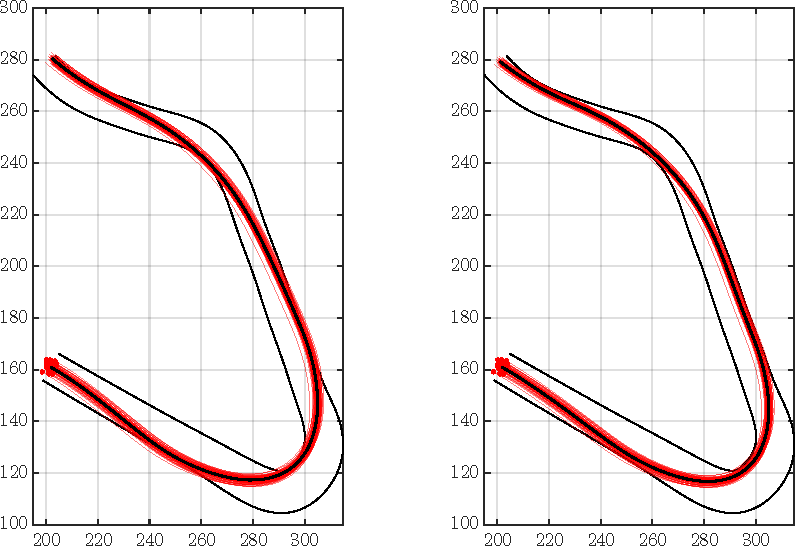
\includegraphics{Fig/olcl_traj_strings.pdf}
	\caption{100 simulations (each panel) with random initial conditions and Gaussian noise realizations. In the left panel, the reference trajectory (black curve) is the non-robust one, tracked using an LQR controller designed around it as per Step 2 of Subsection~\ref{sec:LQR}. In the right panel, the reference (black curve) is a robust trajectory obtained using the closed-loop optimization method as per Step 3 of Subsection~\ref{sec:CLrobustified}, which is tracked using the corresponding optimized controller.}
	\label{fig:traj_strings}
\end{figure}
To provide an empirical validation of the closed-loop robustified planning we simulated the evolution of the controlled vehicle with 100 random initial conditions and included noise realizations. The random values for the initial state and the noise follow a Gaussian distribution with covariance matrices $\bP_0$ and $\bQ$, in both cases, as introduced in Eq.~\eqref{eq:dP}. This analysis is not applicable the open-loop approach, as it does not compute a stabilizing controller---resulting in trajectories that would significantly deviate from the track limits beyond the prediction horizon.
%For visual clarity, the comparison is limited to trajectories with the robustified TLC, but analogous considerations apply to the robustified FLC as well.


The left panel of Fig.~\ref{fig:traj_strings} shows random evolutions (red lines) for an LQR-controlled vehicle stabilized to follow the nominal optimal trajectory (black line). No robust constraints are introduced, and the controller implements the feedback policy from Step 2 of Subsection~\ref{sec:LQR}. The right panel, instead, shows the random evolutions (red lines) for the robustified LQR-based controller obtained in the Step 3 of the closed-loop approach described in Subsection~\ref{sec:CLrobustified}. The corresponding robustified mean trajectory is shown in black.
The comparison between the panels shows that the robustified controller is significantly more effective at satisfying the TLC, resulting in safer and more reliable trajectory tracking.

%---------------------------------
%ORIGINAL VERSION

%This analysis aims to provide empirical validation of the robust trajectories obtained using the methods proposed in this work. For conciseness, the comparison is limited to a nominal trajectory and a trajectory computed using the closed-loop method with only the track limit constraint robustified.
%An LQR controller, designed according to the procedure outlined in Section~\ref{sec:LQR}, is implemented to stabilize the nominal trajectory. In contrast, the robust trajectory is tracked using the controller directly obtained from the optimization process.

